\chapter{Pi-Funktion und Primzahlsatz}

Zur Untersuchung der Verteilungen der Primzahlen betrachtet man unter anderem die Funktion

\begin{equation*}
    \pi:\mathbb{N} \rightarrow \mathbb{N}, n \mapsto \pi(n)
\end{equation*}
die die Anzahl der Primzahlen $\leq n$ angibt und auch \emph{Primzahlzählfunktion} genannt wird.
Z.B. ist 

\begin{equation*}
    \pi(1)=0;\quad \pi(10)=4;\quad \pi(100)=25; \quad \pi(1000)=168;\quad \pi(1000000)=78498
\end{equation*}

Diese Funktion und ihr Wachstumsverhalten ist ein beliebter Forschungsgegenstand in der Zahlentheorie.
Mit der Zeit wurden einige Näherungsformeln entwickelt und verbessert \cite{MopOverview}

Der Primzahlsatz besagt, dass

\begin{equation*}
    \pi(x)\sim\frac x {\ln x}
\end{equation*}

gilt, das heißt, dass der Quotient von linker und rechter Seite für $x \rightarrow \infty$ gegen 1 strebt:

\begin{equation*}
    \lim_{x \rightarrow \infty}\frac{\pi(x)}{\frac{x}{\ln x}}=1
\end{equation*}


\begin{figure}[h]
    \centering
    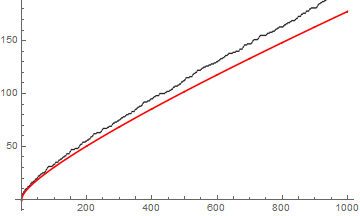
\includegraphics[width=0.5\linewidth]{pi-func.png}
    \caption{Die Pi-Funktion}
    \label{fig:pi-function}
\end{figure}



